\documentclass[tikz]{standalone}
\usepackage{pgfplots}
\usepackage{pgfplotstable}
\pgfplotsset{compat=1.18}
\usepgfplotslibrary{fillbetween} % 1. Load the library

\begin{document}

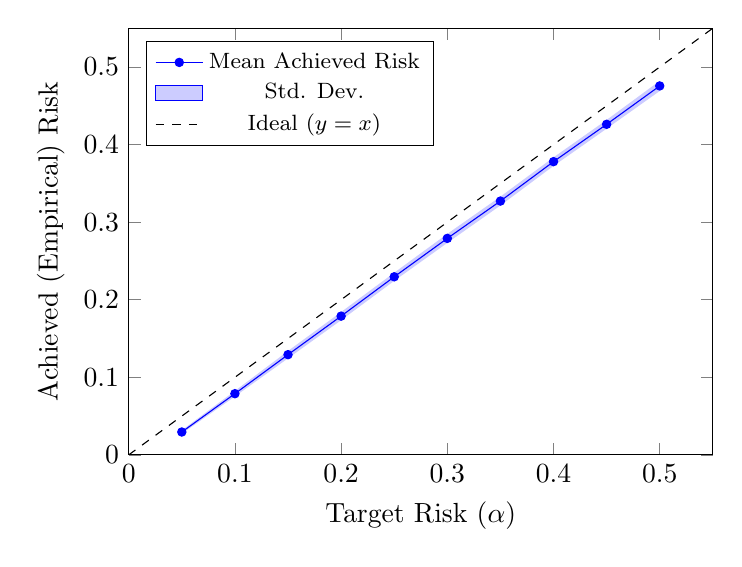
\begin{tikzpicture}
\begin{axis}[
    width=9cm, height=7cm,
    xlabel={Target Risk (\(\alpha\))},
    ylabel={Achieved (Empirical) Risk},
    xmin=0, xmax=0.55,
    ymin=0, ymax=0.55,
    legend style={
        font=\footnotesize,
    },
    legend pos=north west,
    % Ensure the axis lines are drawn on top of the fill
    axis on top,
]

% Define the data source to avoid repetition
\pgfplotstableread{
x y y-err
0.05 0.02947 0.00217
0.10 0.07888 0.00353
0.15 0.12918 0.00476
0.20 0.17887 0.00530
0.25 0.22956 0.00527
0.30 0.27908 0.00583
0.35 0.32719 0.00571
0.40 0.37799 0.00553
0.45 0.42613 0.00563
0.50 0.47560 0.00655
}\mydata

\addplot [
    blue,
    mark=*,
    mark size=1.5pt,
] table [x=x, y=y] {\mydata};
\addlegendentry{Mean Achieved Risk}

\addplot [draw=none, name path=upper, forget plot] table [
    x=x,
    y expr={\thisrow{y} + \thisrow{y-err}}
] {\mydata};

\addplot [draw=none, name path=lower, forget plot] table [
    x=x,
    y expr={\thisrow{y} - \thisrow{y-err}}
] {\mydata};

\addplot [blue, fill opacity=0.2, area legend] fill between[of=upper and lower];
\addlegendentry{Std. Dev.}

\addplot [dashed, black, domain=0:0.6] {x};
\addlegendentry{Ideal \((y=x)\)}

\end{axis}
\end{tikzpicture}

\end{document}
